% Niveau :      PCSI
% Discipline :  Ondes signaux
% Mots clés :   Propagation des ondes

\begin{exercise}{Radar routier}{2}{Sup,Spé}
{Ondes,Propagation des ondes,Doppler}{bermudez}

On étudie le principe de fonctionnement d'un radar. On considère la situation suivante où le radar, situé hors agglomération, en $x=0$, regarde un véhicule (en $x<0$) se dirigeant vers lui a la vitesse $v$ (algébrique) : \\[1ex]

\begin{center}
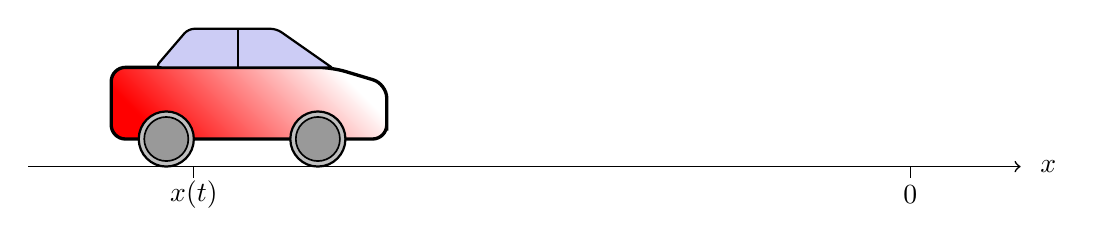
\begin{tikzpicture}[x=-0.7cm,y=0.7cm]
    \shade[top color=red, bottom color=white, shading angle={135}]
        [draw=black,fill=red!20,rounded corners=1.2ex,very thick] (1.5,.5) -- ++(0,1) -- ++(1,0.3) --  ++(3,0) -- ++(1,0) -- ++(0,-1.3) -- (1.5,.5) -- cycle;
    \draw[very thick, rounded corners=0.5ex,fill=black!20!blue!20!white,thick]  (2.5,1.8) -- ++(1,0.7) -- ++(1.6,0) -- ++(0.6,-0.7) -- (2.5,1.8);
    \draw[thick]  (4.2,1.8) -- (4.2,2.5);
    \draw[draw=black,fill=gray!50,thick] (2.75,.5) circle (.5);
    \draw[draw=black,fill=gray!50,thick] (5.5,.5) circle (.5);
    \draw[draw=black,fill=gray!80,semithick] (2.75,.5) circle (.4);
    \draw[draw=black,fill=gray!80,semithick] (5.5,.5) circle (.4);

    \draw[<-,semithick] (-10,0) -- (8,0);
    \draw (-10.5,0) node {$x$};
    \draw (5,0) -- (5,-.2);
    \draw (5,-.5) node {$x(t)$};
    \draw (-8,0) -- (-8,-.2);
    \draw (-8,-.5) node {$0$};
\end{tikzpicture}
\end{center}

Pour cela il envoie un signal $s(t)$.

\begin{questions}
    \questioncours Propagation unidimensionnelle d'une onde progressive. Cas des ondes électromagnétiques dans le vide. Déterminer $s(x,t)$.
    \uplevel{\`A l'instant $t = 0$, l'émetteur envoie un train d'ondes puis un second à
l'instant $t = T$, où $T$ est donc la période d'émission des trains d'ondes. Le signal se réfléchit ensuite sur le véhicule et revient vers le }
    \question Exprimer la période $T'$ perçue par le véhicule.
    \question De même exprimer la période $T''$ perçue par le récepteur du radar et montrer que
    $$f'' = \dfrac{1 + v/c}{1 - v/c}f \stackrel{v \ll c}{\simeq} 1 + 2\dfrac{v}{c}.$$
    \question Le radar envoie un signal sinusoidal de fréquence $f = \SI{24.125}{GHz}$. Interpréter le signal reçu :
\begin{EnvUplevel}
    \centering
    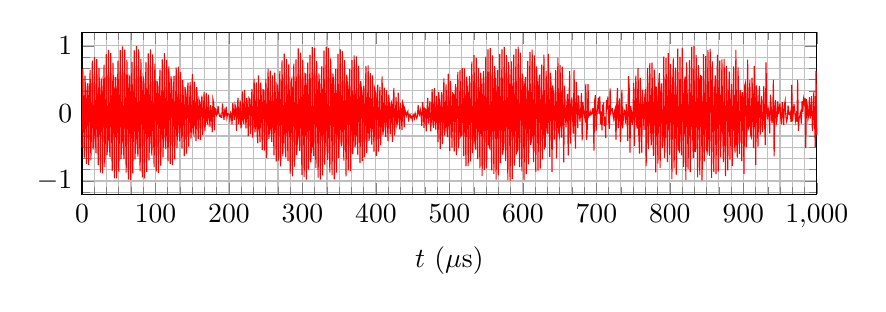
\begin{tikzpicture}
    \begin{axis}[
     clip=false,
     xmin=0,xmax=1000,
     xlabel= $t$ ($\mu$s),
     %axis lines=left,
     %axis x line=middle,
     %axis y line=left,
     width=.9\linewidth,
     height=.3\linewidth,
     ytick={},
     grid=both,
     minor tick num=5,
     ]
      \addplot[domain=0:1000,samples=1000,red]{0.5*sin(deg(x)*1e3)+0.5*sin(deg(x+.3)*(1e3+1.6e-7*24.125*1e3*2*pi))};
      %\addplot[domain=0:1000,samples=200,black,dashed]{cos(deg(x)*1.6e-7*24.125*1e3*pi)};
      %\addplot[domain=0:1000,samples=200,black,dashed]{-cos(deg(x)*1.6e-7*24.125*1e3*pi)};
    \end{axis}
  \end{tikzpicture}
\end{EnvUplevel}
Le véhicule respecte-t-il la limitation en vigueur ?
\uplevel{Pour que le signal soit plus exploitable, on effectue une détection synchrone : le signal reçu $s(t)$ est multiplié par le signal émis $s_0(t)$ et on lui applique un filtre qui coupe les fréquences plus grandes ou égales à $f$.}
    \question Quel est alors ce nouveau signal $g(t)$ ? En quoi ce nouveau signal est plus simple ?
\end{questions}
  

\end{exercise}

\begin{solution}
\begin{questions}
    \question Propagation : $s(x,t) = s(x - ct)$ à droite et $s(x,t) = s(x+ct)$ à gauche.
    \question $T' = \dfrac{1}{1+v/c}T$.
    \question $T'' = (1+v/c)T' = \dfrac{1-v/c}{1+v/c}T$.
    \question 88 km/h
    \question Montage 258
\end{questions}
\end{solution}